\documentclass{./../../Latex/teaching_slides}

\usepackage{venndiagram}
\usepackage{tikz}
\usepackage{pgfplots}
\usetikzlibrary{arrows.meta}

\begin{document}

\title{ECON 441 \\ \vspace{0.4em} \normalsize Introduction to Mathematical Economics}
\author{Div Bhagia}
\date{Lecture 5: Calculus}

\begin{frame}[noframenumbering, plain]
\maketitle
\end{frame}

\begin{frame}{\large (Hypothetical) Production Function for Grades}
\begin{columns}[c]
\begin{column}{0.55\textwidth}
%$$ y = x^2  $$
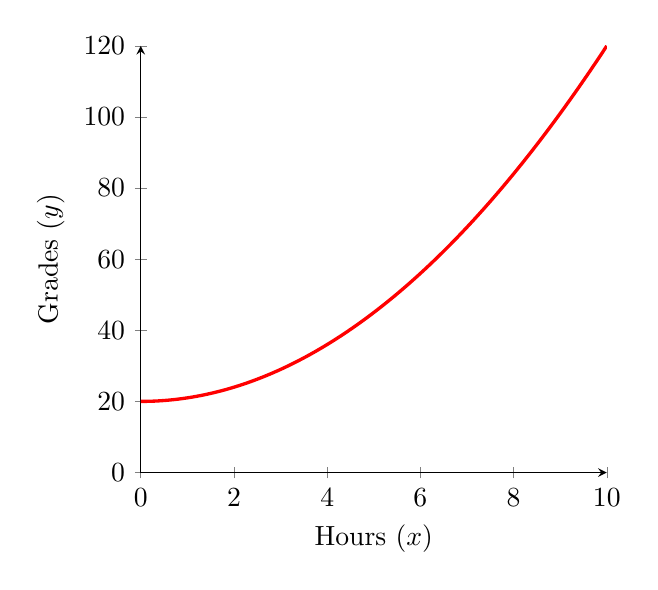
\begin{tikzpicture}
\begin{axis}[
    axis lines = left,
    xlabel = {Hours \((x)\)},
    ylabel = {Grades \((y)\)},
	width = 7.5cm,
	height = 7cm,
	ymin = 0,
]
\addplot [
    domain=-0:10, 
    samples=100, 
    color=red,
	very thick,
    ]
    {x^2 + 20};
\end{axis}
\end{tikzpicture}
\end{column}
\begin{column}{0.45\textwidth}
$$y=f(x)=x^{2}+20$$ \\~\\
How much can your grade can increase if you study for one additional hour per week? \pause \red{Depends on how much you are studying right now!}
\end{column}
\end{columns}
\end{frame}

\begin{frame}{Average Rate of Change}
Use $\Delta$ to denote change:
$$\Delta x=x_{1}-x_{0}$$
Change in $y$ per unit change in $x$:
$$ \frac{\Delta y}{\Delta x}=\frac{f\left(x_{0}+\Delta x\right)-f\left(x_{0}\right)}{\Delta x} $$
\end{frame}

\begin{frame}{Average Rate of Change}
\vspace{-1em}
$$y=f(x)=x^{2}+20$$ 
What happens if you go from 6 to 8 hours of studying? 
$$ x_0 = 6, x_1 = 8 \rightarrow   \Delta x = x_{1}-x_{0}=2 $$
Total change in grades:
$$ f(x_0+\Delta x) - f(x_0) =    $$ 
Per hour change in grade:
$$ \frac{\Delta y}{\Delta x}=\frac{f\left(x_{0}+\Delta x\right)-f\left(x_{0}\right)}{\Delta x} = $$
\end{frame}

\begin{frame}{The Derivative}
%\vspace{1em}
Usually interested in minuscule changes from $x_0$. \\~\\
The derivative of a function is defined as:
$$ \frac{d y}{d x} = f'(x)= \lim_{\Delta x \rightarrow 0} \frac{\Delta y}{\Delta x} $$
\vspace{1em}
Note that $$ \frac{\Delta y}{\Delta x}=\frac{f\left(x_{0}+\Delta x\right)-f\left(x_{0}\right)}{\Delta x}  $$
\end{frame}

\begin{frame}{The Derivative}
%\vspace{1em}
For the function: $y=f(x)=x^{2}+20$
\begin{align*} \frac{\Delta y}{\Delta x}&=\frac{f\left(x_{0}+\Delta x\right)-f\left(x_{0}\right)}{\Delta x} \\
&= \frac{(x_0+\Delta x)^2+20-(x_0^2+20)}{\Delta x} \\
&= \frac{x_0^2+ (\Delta x)^2+2 x_0 \Delta x-x_0^2}{\Delta x} \\&= 2 x_0 + \Delta x
\end{align*} 
Then the derivative is given by: 
$$ \frac{d y}{d x} = f'(x_0)= \lim_{\Delta x \rightarrow 0} 2 x_0 + \Delta x = 2 x_0 $$
\end{frame}

\begin{frame}{The Derivative}
%\vspace{1em}
The derivative:
$$ \frac{d y}{d x} = f'(x_0)= \lim_{\Delta x \rightarrow 0} \frac{f\left(x_{0}+\Delta x\right)-f\left(x_{0}\right)}{\Delta x} $$
\vspace{1em}

Alternatively, 
$$ \frac{d y}{d x} = f'(x_0)= \lim_{ x \rightarrow x_0} \frac{f(x)-f(x_{0})}{x-x_0}  $$
\end{frame}

\begin{frame}{The Derivative}
%\vspace{1em}
For the function: $y=f(x)=x^{2}+20$
\begin{align*} \frac{d y}{d x}&= \lim_{ x \rightarrow x_0} \frac{f(x)-f(x_{0})}{x-x_0} \\
& = \lim_{ x \rightarrow x_0} \frac{x^2+20-x_0^2-20}{x-x_0} \\
& = \lim_{ x \rightarrow x_0} \frac{x^2-x_0^2}{x-x_0} \\
& = \lim_{ x \rightarrow x_0} x+x_0 = 2x_0
\end{align*}
\end{frame}

\begin{frame}{Derivative = Slope of the Tangent Line}
\vspace{-1.5em}
$$y=f(x)=x^{2}+20 \rightarrow f'(x) = 2x$$ 
\centering
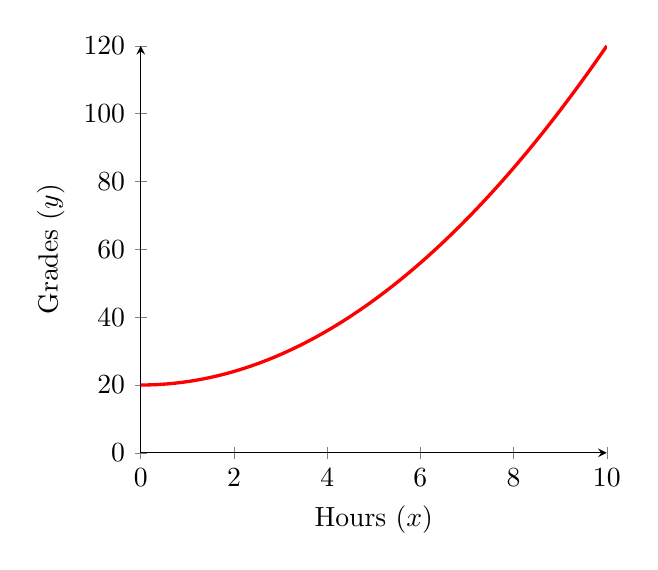
\begin{tikzpicture}
\begin{axis}[
    axis lines = left,
    xlabel = {Hours \((x)\)},
    ylabel = {Grades \((y)\)},
	width = 7.5cm,
	height = 6.75cm,
	ymin = 0,
]
\addplot [
    domain=-0:10, 
    samples=100, 
    color=red,
	very thick,
    ]
    {x^2 + 20};
\end{axis}
\end{tikzpicture}
\end{frame}

\begin{frame}{Concept of a limit}
We say that $L$ is the \textbf{limit} of $f(x)$ at $a$, i.e. $$\lim_{x \rightarrow a} f(x) = L$$
if $f(x)$ approaches $L$ as $x$ approaches $a$ from any direction. \\~\\

Note that we don't actually set $x=a$. \\~\\

Also for the limit to exist at a point we need the function to approach the same value from both directions. 
\end{frame}

\begin{frame}{Concept of a limit}
%We can actually define the limit from both directions separately. \\~\\
\textbf{Left-side limit:} If $x$ approaches $a$ from the left side:
$$\lim_{x \rightarrow a^-} f(x) $$
 \textbf{Right-side limit:} If $x$ approaches $a$ from the right side:
$$\lim_{x \rightarrow a^+} f(x) $$

Only when both left-side and right-side limits have a common finite value, we say that the limit exists. 
 
\end{frame}

\begin{frame}{Example: Limit doesn't exist}
\vspace{1em}
\centering
\includegraphics[scale=0.225]{lim1.png}
\end{frame}

\begin{frame}{Limit: Another example}
$$f(x)\ =\ \frac{4x-4}{\left|x-1\right|} $$
\vspace{1em}

$$\lim_{x \rightarrow 1^-} f(x) = \hspace{8cm} $$ \\

$$\lim_{x \rightarrow 1^+} f(x) = \hspace{8cm} $$

\end{frame}

\begin{frame}{Limit: Another example}
\vspace{1em}
\centering
\includegraphics[scale=0.225]{lim2.png}
\end{frame}


\begin{frame}{Continuity of a Function}
A function $y=f(x)$ is said to be continuous at $a$ if $\lim _{x \rightarrow a} f(x)$ exists and $$\lim _{x \rightarrow a} f(x) = f(a)$$

\end{frame}

\begin{frame}{Discontinuity: Example}
\vspace{1em}
\centering
\begin{columns}[c]
\begin{column}{0.6\textwidth}
\includegraphics[scale=0.225]{cont.png}
\end{column}
\begin{column}{0.4\textwidth}
$$ y = \begin{cases} 2x+1  \text{ if }x<1 \\
2 \text{ if }x=1 \\
2x+1  \text{ if }x>1 \end{cases} $$
\vspace{1em}

In this example, the limit exists but the function is not continuous. 
\end{column} 
\end{columns}
\end{frame}

\begin{frame}{Differentiability and Continuity}
$f'(x_0)$ exists if the following limit exists: 
$$  f'(x_0)= \lim_{ x \rightarrow x_0} \frac{f(x)-f(x_{0})}{x-x_0}  $$


\vspace{1em}
A function $y=f(x)$ is continuous at $x_0$ if $$\lim _{x \rightarrow x_0} f(x) = f(x_0)$$

Any connection? 
\end{frame}

\begin{frame}{Differentiability and Continuity}
Continuity is a necessary condition for differentiability, but it is not sufficient. \\~\\

$f$ is not continuous $\Longrightarrow$ $f$ is not differentiable \\~\\

$f$ is continuous $\Longrightarrow$ $f$ could be differentiable or not \\~\\

\end{frame}

\begin{frame}{Continuous but not differentiable}
\vspace{1em}
\centering
\begin{columns}[c]
\begin{column}{0.6\textwidth}
\includegraphics[scale=0.225]{cont_not_diff.png}
\end{column}
\begin{column}{0.4\textwidth}
$$ y = |x| $$\\

$$ y = \begin{cases} x  \text{ if }x \geq 0  \\
-x \text{ if }x<0 \end{cases} $$
\vspace{1em}

This function is continuous but not differentiable. 
\end{column} 
\end{columns}
\end{frame}

\begin{frame}{So how to differentiate functions?}
Rules of differentiation, easier than taking the limit each time \\~\\
\textit{Constant function rule:}\\
For function \(f(x)=k \), $ f'(x)=0 $.\\~\\
\textit{Power function rule:}\\
For function \( f(x)=x^{n} \), \( f^{\prime}(x)=n x^{n-1} \).\\~\\
\textit{Generalized power function rule:}\\
For function \( f(x)=c x^{n} \), \( f^{\prime}(x)=c n x^{n-1} \).
\end{frame}

\begin{frame}{Rules of Differentiation}
\underline{Two or more functions of one variable} \\~\\ 
\textit{Sum-Difference Rule}
$$ \frac{d}{d x}[f(x) \pm g(x)]=f^{\prime}(x) \pm g^{\prime}(x) $$\\~\\

\textit{Product Rule} \\
$$
\frac{d}{d x}[f(x) g(x)]=f(x) g^{\prime}(x)+f^{\prime}(x) g(x)
$$
\end{frame}

\begin{frame}{Rules of Differentiation}
\underline{Two or more functions of one variable} \\~\\ 
\textit{Quotient Rule}\\
$$ \frac{d}{d x} \frac{f(x)}{g(x)}=\frac{f^{\prime}(x) g(x)-f(x) g^{\prime}(x)}{g(x)^2} $$\\~\\
\textit{Inverse Function Rule}
$$
\frac{d x}{d y}=\frac{1}{d y / d x}
$$

\end{frame}


\begin{frame}{Rules of Differentiation}
\underline{Functions of Different Variables} \\~\\
\textit{Chain Rule} \\
\vspace{0.5em}
For \( z=f(y), \quad y=g(x) \)
$$ \frac{d z}{d x}=\frac{d z}{d y} \cdot \frac{d y}{d x}=f^{\prime}(y) g^{\prime}(x) $$ \\~\\
\end{frame}

\begin{frame}{References and Homework}
Textbook Reference: Sections 6.2-6.4, 6.7, 7.1-7.3 \\~\\
Homework Questions: \\ \vspace{0.5em}
\begin{witemize}
  \item Exercise 6.2: 2,3
  \item Exercise 7.1: 3
  \item Exercise 7.2: 3 (d) (e), 7, 8
  \item Exercise 7.3: 1-6
\end{witemize}
\end{frame}


\begin{comment}
\begin{frame}{How to solve an inequality?}

\end{frame}




\begin{frame}{Double derivative}
Double derivative
\end{frame}


\begin{frame}{Rules of Inequalities}
Transitivity:
$$a>b, b>c \Longrightarrow a>c$$
$$a\geq b, b\geq c \Longrightarrow a \geq c$$ \\~\\

Addition and Subtraction:
$$ a>b \Longrightarrow a \pm k>b \pm k $$
$$a \geq b \Longrightarrow a \pm k \geq b \pm k$$

\end{frame}


\begin{frame}{Rules of Inequalities}
Multiplication and Division:

$$a>b \Longrightarrow k a>k b \quad if \quad k>0 $$
$$a>b \Longrightarrow k a<k b \quad if \quad k<0 $$ \\~\\

Squaring:
$$a>b \geq 0 \Longrightarrow a^{2}>b^{2} $$
\end{frame}

\begin{frame}{Absolute Values and Inequalities}
For any real number $n$, the absolute value of $n$ is given by:

$$
|n|= \begin{cases}n & \text { if } n>0 \\ -n & \text { if } n<0 \\ 0 & \text { if } n=0\end{cases}
$$
\vspace{1em}

What does $x<|n|$ mean? 
\end{frame}

\begin{frame}{Properties of Absolute Values}
The following properties characterize absolute values:

 $$|m|+|n| \geq|m+n|$$

 $$|m| \cdot|n|=|m \cdot n|$$

 $$\frac{|m|}{|n|}=\left|\frac{m}{n}\right|$$
\end{frame}

\begin{frame}{Limit Theorems}
Theorem I: If $q=a v+b$, then $\lim _{v \rightarrow N} q=a N+b$.

Theorem II: If $q=g(v)=b$, then $\lim _{v \rightarrow N} q=b$.

Theorem III: $\lim _{v \rightarrow N} v^{k}=N^{k}$.

Theorem IV: $\lim _{v \rightarrow N}\left(q_{1}+q_{2}\right)=L_{1}+L_{2}$. Theorem V: $\lim _{v \rightarrow N}\left(q_{1} q_{2}\right)=L_{1} L_{2}$

Theorem VI: $\lim _{v \rightarrow N} \frac{q_{1}}{q_{2}}=\frac{L_{1}}{L_{2}}\left(L_{2} \neq 0\right)$.

\end{frame}
\end{comment}

\end{document}